\documentclass[letterpaper,9pt,twoside,printwatermark=false]{pinp}

%% Some pieces required from the pandoc template
\providecommand{\tightlist}{%
  \setlength{\itemsep}{0pt}\setlength{\parskip}{0pt}}

% Use the lineno option to display guide line numbers if required.
% Note that the use of elements such as single-column equations
% may affect the guide line number alignment.

\usepackage[T1]{fontenc}
\usepackage[utf8]{inputenc}

% The geometry package layout settings need to be set here...
\geometry{layoutsize={0.95588\paperwidth,0.98864\paperheight},%
          layouthoffset=0.02206\paperwidth,%
		  layoutvoffset=0.00568\paperheight}

\definecolor{pinpblue}{HTML}{185FAF}  % imagecolorpicker on blue for new R logo
\definecolor{pnasbluetext}{RGB}{101,0,0} %



\title{Exercise 1 - How Deep is the Ocean? September 17, 2018.}

\author[a]{EPIB607 - Inferential Statistics}

  \affil[a]{Fall 2018, McGill University}

\setcounter{secnumdepth}{5}

% Please give the surname of the lead author for the running footer
\leadauthor{Bhatnagar and Hanley}

% Keywords are not mandatory, but authors are strongly encouraged to provide them. If provided, please include two to five keywords, separated by the pipe symbol, e.g:
 \keywords{  Sampling distribution |  Means |  Proportions |  Standard error |  Standard deviation |  Parameter |  Statistic  }  

\begin{abstract}
This in-class exercise will introduce you to sampling distributions for
means and proportions.
\end{abstract}

\dates{This version was compiled on \today}
\doi{\url{https://sahirbhatnagar.com/EPIB607/}}

\pinpfootercontents{Exercise 1: Sampling Distributions for Means and Proportions}

\begin{document}

% Optional adjustment to line up main text (after abstract) of first page with line numbers, when using both lineno and twocolumn options.
% You should only change this length when you've finalised the article contents.
\verticaladjustment{-2pt}

\maketitle
\thispagestyle{firststyle}
\ifthenelse{\boolean{shortarticle}}{\ifthenelse{\boolean{singlecolumn}}{\abscontentformatted}{\abscontent}}{}

% If your first paragraph (i.e. with the \dropcap) contains a list environment (quote, quotation, theorem, definition, enumerate, itemize...), the line after the list may have some extra indentation. If this is the case, add \parshape=0 to the end of the list environment.


\section{What percentage of the world's surface is covered by
water?}\label{what-percentage-of-the-worlds-surface-is-covered-by-water}

The data provided by the
\href{https://topex.ucsd.edu/cgi-bin/get_srtm30.cgi}{Scripps Institution
of Oceanography} can provide an answer, but some work is required on
your part. James Hanley (JH) has randomly sampled \(n=5\) and \(n=20\)
latitudes and longitudes for every student in the class. This document
contains unique latitudes and longitudes for

\begin{ShadedResult}
\begin{verbatim}
[1] "Bhatnagar, Sahir"
\end{verbatim}
\end{ShadedResult}

and was sent in an email (using the
\href{https://cran.r-project.org/package=gmailr}{gmailr} package) as a
pdf attachment to the following address:

\begin{ShadedResult}
\begin{verbatim}
[1] "sahir.bhatnagar@mcgill.ca"
\end{verbatim}
\end{ShadedResult}

\subsection*{A sample of 5}\label{a-sample-of-5}
\addcontentsline{toc}{subsection}{A sample of 5}

\begin{ShadedResult}
\begin{verbatim}
Latitude.n.5 <- c(8.042,45.329,37.743,-12.237,21.552)
\end{verbatim}
\end{ShadedResult}\begin{ShadedResult}
\begin{verbatim}
Longitude.n.5 <- c(35.241,125.735,-134.383,-23.623,-5.339)
\end{verbatim}
\end{ShadedResult}

\subsection*{A sample of 20}\label{a-sample-of-20}
\addcontentsline{toc}{subsection}{A sample of 20}

\begin{ShadedResult}
\begin{verbatim}
Latitude.n.20 <- c(40.428,59.851,-38.35,-8.862,-26.312,-49.721,-4.02,44.028,-36.308,22.071,
44.765,-18.818,37.185,41.768,-5.255,14.199,61.165,10.874,-27.083,15.792)
\end{verbatim}
\end{ShadedResult}\begin{ShadedResult}
\begin{verbatim}
Longitude.n.20 <- c(57.814,40.026,131.012,-145.304,-130.685,48.011,59.257,111.303,41.137,-61.05,
159.666,-110.195,-87.961,-118.8,99.592,-102.281,159.827,-166.667,-2.171,-6.664)
\end{verbatim}
\end{ShadedResult}

\subsection{Determine the proportion of water from the sample of
5}\label{determine-the-proportion-of-water-from-the-sample-of-5}

\begin{enumerate}
\def\labelenumi{\arabic{enumi}.}
\tightlist
\item
  Using the sample of 5, manually enter the latitudes and longitudes in
  \href{https://www.google.com/maps}{Google maps} and record if you land
  on water or land. Figure\ref{maps} shows how to enter them.
\end{enumerate}

\begin{figure}[H]
  \begin{center}
    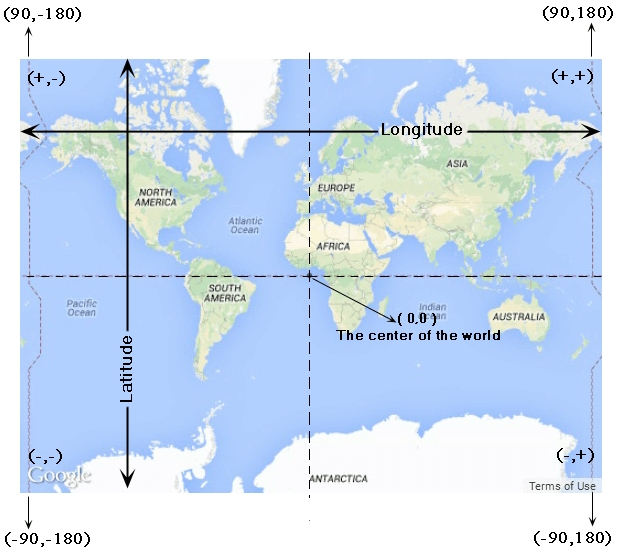
\includegraphics[scale=0.40]{lat-long.png} 
  \end{center}
  \caption{Latitude and longitude in Google maps. Latitudes range from (-90,90) and longitudes range from (-180, 180). Latitude is entered first followed by longitude and separated by a comma.}\label{maps}
\end{figure}

\begin{enumerate}
\def\labelenumi{\arabic{enumi}.}
\setcounter{enumi}{1}
\tightlist
\item
  In \texttt{R}, store your results in a binary vector of length 5. For
  example, if your sample landed on water 3 times out of 5, then you
  would enter the following in \texttt{R} (1 for water and 0 for land):
\end{enumerate}

\begin{ShadedResult}
\begin{verbatim}
landed_in_water <- c(1,1,1,0,0)
\end{verbatim}
\end{ShadedResult}

\begin{enumerate}
\def\labelenumi{\arabic{enumi}.}
\setcounter{enumi}{2}
\item
  Using \texttt{R}, estimate the percentage of the world's surface
  covered by water from your sample of 5. This can be done by simply
  taking the mean of the binary vector created in Step 2:
  \texttt{mean(landed\_in\_water)}.
\item
  Enter your estimate in this
  \href{https://docs.google.com/spreadsheets/d/1Mnxeq9nQcTdQycZ7S_62fYFiNC5_a3fibsyodzfwO58/edit?usp=sharing}{Google
  sheet} next to your name and in the column titled
  \texttt{PropnW.5.locations}.
\end{enumerate}

\subsection{Determine the proportion of water from the sample of
20}\label{determine-the-proportion-of-water-from-the-sample-of-20}

\begin{enumerate}
\def\labelenumi{\arabic{enumi}.}
\tightlist
\item
  Repeat the above steps for the sample of 20. \textbf{Before you do},
  take a moment to think about how tedious a process it can be to
  manually enter 20 latitudes and longitudes into Google maps. JH and SB
  hope you can appreciate the parallels between this toy exercise and
  that of collecting data for your research projects, i.e., it becomes
  increasingly difficult to collect more and more samples.
\end{enumerate}

Now that you appreciate the amount of work it takes to estimate the
proportion of water from 20 samples, JH and SB think it is sufficient
for you to use some automatic procedures to complete this task, which
are further described in step 2.

\begin{enumerate}
\def\labelenumi{\arabic{enumi}.}
\setcounter{enumi}{1}
\tightlist
\item
  Create an \texttt{R} script and copy paste the following index vector
  into it:
\end{enumerate}

\begin{ShadedResult}
\begin{verbatim}
index.n.20 <- c(2131,2132,2133,2134,2135,2136,2137,2138,2139,2140,
2141,2142,2143,2144,2145,2146,2147,2148,2149,2150)
\end{verbatim}
\end{ShadedResult}

%\showmatmethods


\bibliography{pinp}
\bibliographystyle{jss}



\end{document}

